% Options for packages loaded elsewhere
\PassOptionsToPackage{unicode}{hyperref}
\PassOptionsToPackage{hyphens}{url}
%
\documentclass[
]{article}
\usepackage{lmodern}
\usepackage{amssymb,amsmath}
\usepackage{ifxetex,ifluatex}
\ifnum 0\ifxetex 1\fi\ifluatex 1\fi=0 % if pdftex
  \usepackage[T1]{fontenc}
  \usepackage[utf8]{inputenc}
  \usepackage{textcomp} % provide euro and other symbols
\else % if luatex or xetex
  \usepackage{unicode-math}
  \defaultfontfeatures{Scale=MatchLowercase}
  \defaultfontfeatures[\rmfamily]{Ligatures=TeX,Scale=1}
\fi
% Use upquote if available, for straight quotes in verbatim environments
\IfFileExists{upquote.sty}{\usepackage{upquote}}{}
\IfFileExists{microtype.sty}{% use microtype if available
  \usepackage[]{microtype}
  \UseMicrotypeSet[protrusion]{basicmath} % disable protrusion for tt fonts
}{}
\makeatletter
\@ifundefined{KOMAClassName}{% if non-KOMA class
  \IfFileExists{parskip.sty}{%
    \usepackage{parskip}
  }{% else
    \setlength{\parindent}{0pt}
    \setlength{\parskip}{6pt plus 2pt minus 1pt}}
}{% if KOMA class
  \KOMAoptions{parskip=half}}
\makeatother
\usepackage{xcolor}
\IfFileExists{xurl.sty}{\usepackage{xurl}}{} % add URL line breaks if available
\IfFileExists{bookmark.sty}{\usepackage{bookmark}}{\usepackage{hyperref}}
\hypersetup{
  pdftitle={CourseraRepRes RepData\_PeerAssessment1},
  pdfauthor={E.C.},
  hidelinks,
  pdfcreator={LaTeX via pandoc}}
\urlstyle{same} % disable monospaced font for URLs
\usepackage[margin=1in]{geometry}
\usepackage{color}
\usepackage{fancyvrb}
\newcommand{\VerbBar}{|}
\newcommand{\VERB}{\Verb[commandchars=\\\{\}]}
\DefineVerbatimEnvironment{Highlighting}{Verbatim}{commandchars=\\\{\}}
% Add ',fontsize=\small' for more characters per line
\usepackage{framed}
\definecolor{shadecolor}{RGB}{248,248,248}
\newenvironment{Shaded}{\begin{snugshade}}{\end{snugshade}}
\newcommand{\AlertTok}[1]{\textcolor[rgb]{0.94,0.16,0.16}{#1}}
\newcommand{\AnnotationTok}[1]{\textcolor[rgb]{0.56,0.35,0.01}{\textbf{\textit{#1}}}}
\newcommand{\AttributeTok}[1]{\textcolor[rgb]{0.77,0.63,0.00}{#1}}
\newcommand{\BaseNTok}[1]{\textcolor[rgb]{0.00,0.00,0.81}{#1}}
\newcommand{\BuiltInTok}[1]{#1}
\newcommand{\CharTok}[1]{\textcolor[rgb]{0.31,0.60,0.02}{#1}}
\newcommand{\CommentTok}[1]{\textcolor[rgb]{0.56,0.35,0.01}{\textit{#1}}}
\newcommand{\CommentVarTok}[1]{\textcolor[rgb]{0.56,0.35,0.01}{\textbf{\textit{#1}}}}
\newcommand{\ConstantTok}[1]{\textcolor[rgb]{0.00,0.00,0.00}{#1}}
\newcommand{\ControlFlowTok}[1]{\textcolor[rgb]{0.13,0.29,0.53}{\textbf{#1}}}
\newcommand{\DataTypeTok}[1]{\textcolor[rgb]{0.13,0.29,0.53}{#1}}
\newcommand{\DecValTok}[1]{\textcolor[rgb]{0.00,0.00,0.81}{#1}}
\newcommand{\DocumentationTok}[1]{\textcolor[rgb]{0.56,0.35,0.01}{\textbf{\textit{#1}}}}
\newcommand{\ErrorTok}[1]{\textcolor[rgb]{0.64,0.00,0.00}{\textbf{#1}}}
\newcommand{\ExtensionTok}[1]{#1}
\newcommand{\FloatTok}[1]{\textcolor[rgb]{0.00,0.00,0.81}{#1}}
\newcommand{\FunctionTok}[1]{\textcolor[rgb]{0.00,0.00,0.00}{#1}}
\newcommand{\ImportTok}[1]{#1}
\newcommand{\InformationTok}[1]{\textcolor[rgb]{0.56,0.35,0.01}{\textbf{\textit{#1}}}}
\newcommand{\KeywordTok}[1]{\textcolor[rgb]{0.13,0.29,0.53}{\textbf{#1}}}
\newcommand{\NormalTok}[1]{#1}
\newcommand{\OperatorTok}[1]{\textcolor[rgb]{0.81,0.36,0.00}{\textbf{#1}}}
\newcommand{\OtherTok}[1]{\textcolor[rgb]{0.56,0.35,0.01}{#1}}
\newcommand{\PreprocessorTok}[1]{\textcolor[rgb]{0.56,0.35,0.01}{\textit{#1}}}
\newcommand{\RegionMarkerTok}[1]{#1}
\newcommand{\SpecialCharTok}[1]{\textcolor[rgb]{0.00,0.00,0.00}{#1}}
\newcommand{\SpecialStringTok}[1]{\textcolor[rgb]{0.31,0.60,0.02}{#1}}
\newcommand{\StringTok}[1]{\textcolor[rgb]{0.31,0.60,0.02}{#1}}
\newcommand{\VariableTok}[1]{\textcolor[rgb]{0.00,0.00,0.00}{#1}}
\newcommand{\VerbatimStringTok}[1]{\textcolor[rgb]{0.31,0.60,0.02}{#1}}
\newcommand{\WarningTok}[1]{\textcolor[rgb]{0.56,0.35,0.01}{\textbf{\textit{#1}}}}
\usepackage{longtable,booktabs}
% Correct order of tables after \paragraph or \subparagraph
\usepackage{etoolbox}
\makeatletter
\patchcmd\longtable{\par}{\if@noskipsec\mbox{}\fi\par}{}{}
\makeatother
% Allow footnotes in longtable head/foot
\IfFileExists{footnotehyper.sty}{\usepackage{footnotehyper}}{\usepackage{footnote}}
\makesavenoteenv{longtable}
\usepackage{graphicx,grffile}
\makeatletter
\def\maxwidth{\ifdim\Gin@nat@width>\linewidth\linewidth\else\Gin@nat@width\fi}
\def\maxheight{\ifdim\Gin@nat@height>\textheight\textheight\else\Gin@nat@height\fi}
\makeatother
% Scale images if necessary, so that they will not overflow the page
% margins by default, and it is still possible to overwrite the defaults
% using explicit options in \includegraphics[width, height, ...]{}
\setkeys{Gin}{width=\maxwidth,height=\maxheight,keepaspectratio}
% Set default figure placement to htbp
\makeatletter
\def\fps@figure{htbp}
\makeatother
\setlength{\emergencystretch}{3em} % prevent overfull lines
\providecommand{\tightlist}{%
  \setlength{\itemsep}{0pt}\setlength{\parskip}{0pt}}
\setcounter{secnumdepth}{-\maxdimen} % remove section numbering

\title{CourseraRepRes RepData\_PeerAssessment1}
\author{E.C.}
\date{}

\begin{document}
\maketitle

\hypertarget{introinstructions-for-reference-code-below}{%
\subsection{Intro/Instructions for reference (code
below)}\label{introinstructions-for-reference-code-below}}

It is now possible to collect a large amount of data about personal
movement using activity monitoring devices such as a Fitbit, Nike
Fuelband, or Jawbone Up. These type of devices are part of the
``quantified self'' movement -- a group of enthusiasts who take
measurements about themselves regularly to improve their health, to find
patterns in their behavior, or because they are tech geeks. But these
data remain under-utilized both because the raw data are hard to obtain
and there is a lack of statistical methods and software for processing
and interpreting the data.

This assignment makes use of data from a personal activity monitoring
device. This device collects data at 5 minute intervals through out the
day. The data consists of two months of data from an anonymous
individual collected during the months of October and November, 2012 and
include the number of steps taken in 5 minute intervals each day.

The data for this assignment can be downloaded from the course web site:

\begin{itemize}
\tightlist
\item
  Dataset:
  \href{https://d396qusza40orc.cloudfront.net/repdata\%2Fdata\%2Factivity.zip}{Activity
  monitoring data}
\end{itemize}

The variables included in this dataset are:

steps: Number of steps taking in a 5-minute interval (missing values are
coded as 𝙽𝙰) date: The date on which the measurement was taken in
YYYY-MM-DD format interval: Identifier for the 5-minute interval in
which measurement was taken The dataset is stored in a
comma-separated-value (CSV) file and there are a total of 17,568
observations in this dataset.

\hypertarget{loading-and-preprocessing-the-data}{%
\subsection{Loading and preprocessing the
data}\label{loading-and-preprocessing-the-data}}

Unzip data to obtain a csv file.

\begin{Shaded}
\begin{Highlighting}[]
\KeywordTok{library}\NormalTok{(}\StringTok{"data.table"}\NormalTok{)}
\KeywordTok{library}\NormalTok{(ggplot2)}

\NormalTok{fileUrl <-}\StringTok{ "https://d396qusza40orc.cloudfront.net/repdata%2Fdata%2Factivity.zip"}
\KeywordTok{download.file}\NormalTok{(fileUrl, }\DataTypeTok{destfile =} \KeywordTok{paste0}\NormalTok{(}\KeywordTok{getwd}\NormalTok{(), }\StringTok{'/repdata%2Fdata%2Factivity.zip'}\NormalTok{), }\DataTypeTok{method =} \StringTok{"curl"}\NormalTok{)}
\KeywordTok{unzip}\NormalTok{(}\StringTok{"repdata%2Fdata%2Factivity.zip"}\NormalTok{,}\DataTypeTok{exdir =} \StringTok{"data"}\NormalTok{)}
\end{Highlighting}
\end{Shaded}

\hypertarget{reading-csv-data-into-data.table.}{%
\subsection{Reading csv Data into
Data.Table.}\label{reading-csv-data-into-data.table.}}

\begin{Shaded}
\begin{Highlighting}[]
\NormalTok{activityDT <-}\StringTok{ }\NormalTok{data.table}\OperatorTok{::}\KeywordTok{fread}\NormalTok{(}\DataTypeTok{input =} \StringTok{"data/activity.csv"}\NormalTok{)}
\end{Highlighting}
\end{Shaded}

\hypertarget{what-is-mean-total-number-of-steps-taken-per-day}{%
\subsection{What is mean total number of steps taken per
day?}\label{what-is-mean-total-number-of-steps-taken-per-day}}

\begin{enumerate}
\def\labelenumi{\arabic{enumi}.}
\tightlist
\item
  Calculate the total number of steps taken per day
\end{enumerate}

\begin{Shaded}
\begin{Highlighting}[]
\NormalTok{Total_Steps <-}\StringTok{ }\NormalTok{activityDT[, }\KeywordTok{c}\NormalTok{(}\KeywordTok{lapply}\NormalTok{(.SD, sum, }\DataTypeTok{na.rm =} \OtherTok{FALSE}\NormalTok{)), .SDcols =}\StringTok{ }\KeywordTok{c}\NormalTok{(}\StringTok{"steps"}\NormalTok{), by =}\StringTok{ }\NormalTok{.(date)] }

\KeywordTok{head}\NormalTok{(Total_Steps, }\DecValTok{10}\NormalTok{)}
\end{Highlighting}
\end{Shaded}

\begin{verbatim}
##           date steps
##  1: 2012-10-01    NA
##  2: 2012-10-02   126
##  3: 2012-10-03 11352
##  4: 2012-10-04 12116
##  5: 2012-10-05 13294
##  6: 2012-10-06 15420
##  7: 2012-10-07 11015
##  8: 2012-10-08    NA
##  9: 2012-10-09 12811
## 10: 2012-10-10  9900
\end{verbatim}

\begin{enumerate}
\def\labelenumi{\arabic{enumi}.}
\setcounter{enumi}{1}
\tightlist
\item
  If you do not understand the difference between a histogram and a
  barplot, research the difference between them. Make a histogram of the
  total number of steps taken each day.
\end{enumerate}

\begin{Shaded}
\begin{Highlighting}[]
\KeywordTok{ggplot}\NormalTok{(Total_Steps, }\KeywordTok{aes}\NormalTok{(}\DataTypeTok{x =}\NormalTok{ steps)) }\OperatorTok{+}
\StringTok{    }\KeywordTok{geom_histogram}\NormalTok{(}\DataTypeTok{fill =} \StringTok{"blue"}\NormalTok{, }\DataTypeTok{binwidth =} \DecValTok{1000}\NormalTok{) }\OperatorTok{+}
\StringTok{    }\KeywordTok{labs}\NormalTok{(}\DataTypeTok{title =} \StringTok{"Daily Steps"}\NormalTok{, }\DataTypeTok{x =} \StringTok{"Steps"}\NormalTok{, }\DataTypeTok{y =} \StringTok{"Frequency"}\NormalTok{)}
\end{Highlighting}
\end{Shaded}

\begin{verbatim}
## Warning: Removed 8 rows containing non-finite values (stat_bin).
\end{verbatim}

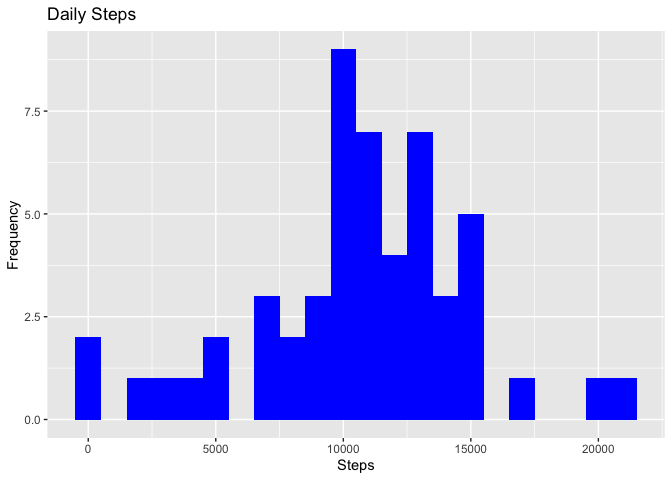
\includegraphics{PA1_template_files/figure-latex/unnamed-chunk-4-1.pdf}

\begin{enumerate}
\def\labelenumi{\arabic{enumi}.}
\setcounter{enumi}{2}
\tightlist
\item
  Calculate and report the mean and median of the total number of steps
  taken per day
\end{enumerate}

\begin{Shaded}
\begin{Highlighting}[]
\NormalTok{Total_Steps[, .(}\DataTypeTok{Mean_Steps =} \KeywordTok{mean}\NormalTok{(steps, }\DataTypeTok{na.rm =} \OtherTok{TRUE}\NormalTok{), }\DataTypeTok{Median_Steps =} \KeywordTok{median}\NormalTok{(steps, }\DataTypeTok{na.rm =} \OtherTok{TRUE}\NormalTok{))]}
\end{Highlighting}
\end{Shaded}

\begin{verbatim}
##    Mean_Steps Median_Steps
## 1:   10766.19        10765
\end{verbatim}

\hypertarget{what-is-the-average-daily-activity-pattern}{%
\subsection{What is the average daily activity
pattern?}\label{what-is-the-average-daily-activity-pattern}}

\begin{enumerate}
\def\labelenumi{\arabic{enumi}.}
\tightlist
\item
  Make a time series plot (i.e.~𝚝𝚢𝚙𝚎 = ``𝚕'') of the 5-minute interval
  (x-axis) and the average number of steps taken, averaged across all
  days (y-axis)
\end{enumerate}

\begin{Shaded}
\begin{Highlighting}[]
\NormalTok{IntervalDT <-}\StringTok{ }\NormalTok{activityDT[, }\KeywordTok{c}\NormalTok{(}\KeywordTok{lapply}\NormalTok{(.SD, mean, }\DataTypeTok{na.rm =} \OtherTok{TRUE}\NormalTok{)), .SDcols =}\StringTok{ }\KeywordTok{c}\NormalTok{(}\StringTok{"steps"}\NormalTok{), by =}\StringTok{ }\NormalTok{.(interval)] }

\KeywordTok{ggplot}\NormalTok{(IntervalDT, }\KeywordTok{aes}\NormalTok{(}\DataTypeTok{x =}\NormalTok{ interval , }\DataTypeTok{y =}\NormalTok{ steps)) }\OperatorTok{+}\StringTok{ }\KeywordTok{geom_line}\NormalTok{(}\DataTypeTok{color=}\StringTok{"blue"}\NormalTok{, }\DataTypeTok{size=}\DecValTok{1}\NormalTok{) }\OperatorTok{+}\StringTok{ }\KeywordTok{labs}\NormalTok{(}\DataTypeTok{title =} \StringTok{"Avg. Daily Steps"}\NormalTok{, }\DataTypeTok{x =} \StringTok{"Interval"}\NormalTok{, }\DataTypeTok{y =} \StringTok{"Avg. Steps per day"}\NormalTok{)}
\end{Highlighting}
\end{Shaded}

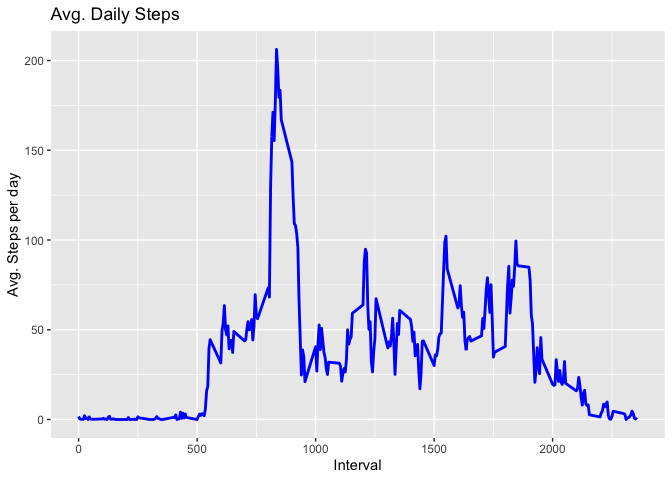
\includegraphics{PA1_template_files/figure-latex/unnamed-chunk-6-1.pdf}

\begin{enumerate}
\def\labelenumi{\arabic{enumi}.}
\setcounter{enumi}{1}
\tightlist
\item
  Which 5-minute interval, on average across all the days in the
  dataset, contains the maximum number of steps?
\end{enumerate}

\begin{Shaded}
\begin{Highlighting}[]
\NormalTok{IntervalDT[steps }\OperatorTok{==}\StringTok{ }\KeywordTok{max}\NormalTok{(steps), .(}\DataTypeTok{max_interval =}\NormalTok{ interval)]}
\end{Highlighting}
\end{Shaded}

\begin{verbatim}
##    max_interval
## 1:          835
\end{verbatim}

\hypertarget{imputing-missing-values}{%
\subsection{Imputing missing values}\label{imputing-missing-values}}

\begin{enumerate}
\def\labelenumi{\arabic{enumi}.}
\tightlist
\item
  Calculate and report the total number of missing values in the dataset
  (i.e.~the total number of rows with 𝙽𝙰s)
\end{enumerate}

\begin{Shaded}
\begin{Highlighting}[]
\NormalTok{activityDT[}\KeywordTok{is.na}\NormalTok{(steps), .N ]}
\end{Highlighting}
\end{Shaded}

\begin{verbatim}
## [1] 2304
\end{verbatim}

\begin{Shaded}
\begin{Highlighting}[]
\CommentTok{# alternative solution}
\KeywordTok{nrow}\NormalTok{(activityDT[}\KeywordTok{is.na}\NormalTok{(steps),])}
\end{Highlighting}
\end{Shaded}

\begin{verbatim}
## [1] 2304
\end{verbatim}

\begin{enumerate}
\def\labelenumi{\arabic{enumi}.}
\setcounter{enumi}{1}
\tightlist
\item
  Devise a strategy for filling in all of the missing values in the
  dataset. The strategy does not need to be sophisticated. For example,
  you could use the mean/median for that day, or the mean for that
  5-minute interval, etc.
\end{enumerate}

\begin{Shaded}
\begin{Highlighting}[]
\CommentTok{# Filling in missing values with median of dataset. }
\NormalTok{activityDT[}\KeywordTok{is.na}\NormalTok{(steps), }\StringTok{"steps"}\NormalTok{] <-}\StringTok{ }\NormalTok{activityDT[, }\KeywordTok{c}\NormalTok{(}\KeywordTok{lapply}\NormalTok{(.SD, median, }\DataTypeTok{na.rm =} \OtherTok{TRUE}\NormalTok{)), .SDcols =}\StringTok{ }\KeywordTok{c}\NormalTok{(}\StringTok{"steps"}\NormalTok{)]}
\end{Highlighting}
\end{Shaded}

\begin{enumerate}
\def\labelenumi{\arabic{enumi}.}
\setcounter{enumi}{2}
\tightlist
\item
  Create a new dataset that is equal to the original dataset but with
  the missing data filled in.
\end{enumerate}

\begin{Shaded}
\begin{Highlighting}[]
\NormalTok{data.table}\OperatorTok{::}\KeywordTok{fwrite}\NormalTok{(}\DataTypeTok{x =}\NormalTok{ activityDT, }\DataTypeTok{file =} \StringTok{"data/tidyData.csv"}\NormalTok{, }\DataTypeTok{quote =} \OtherTok{FALSE}\NormalTok{)}
\end{Highlighting}
\end{Shaded}

\begin{enumerate}
\def\labelenumi{\arabic{enumi}.}
\setcounter{enumi}{3}
\tightlist
\item
  Make a histogram of the total number of steps taken each day and
  calculate and report the mean and median total number of steps taken
  per day. Do these values differ from the estimates from the first part
  of the assignment? What is the impact of imputing missing data on the
  estimates of the total daily number of steps?
\end{enumerate}

\begin{Shaded}
\begin{Highlighting}[]
\CommentTok{# total number of steps taken per day}
\NormalTok{Total_Steps <-}\StringTok{ }\NormalTok{activityDT[, }\KeywordTok{c}\NormalTok{(}\KeywordTok{lapply}\NormalTok{(.SD, sum)), .SDcols =}\StringTok{ }\KeywordTok{c}\NormalTok{(}\StringTok{"steps"}\NormalTok{), by =}\StringTok{ }\NormalTok{.(date)] }

\CommentTok{# mean and median total number of steps taken per day}
\NormalTok{Total_Steps[, .(}\DataTypeTok{Mean_Steps =} \KeywordTok{mean}\NormalTok{(steps), }\DataTypeTok{Median_Steps =} \KeywordTok{median}\NormalTok{(steps))]}
\end{Highlighting}
\end{Shaded}

\begin{verbatim}
##    Mean_Steps Median_Steps
## 1:    9354.23        10395
\end{verbatim}

\begin{Shaded}
\begin{Highlighting}[]
\KeywordTok{ggplot}\NormalTok{(Total_Steps, }\KeywordTok{aes}\NormalTok{(}\DataTypeTok{x =}\NormalTok{ steps)) }\OperatorTok{+}\StringTok{ }\KeywordTok{geom_histogram}\NormalTok{(}\DataTypeTok{fill =} \StringTok{"blue"}\NormalTok{, }\DataTypeTok{binwidth =} \DecValTok{1000}\NormalTok{) }\OperatorTok{+}\StringTok{ }\KeywordTok{labs}\NormalTok{(}\DataTypeTok{title =} \StringTok{"Daily Steps"}\NormalTok{, }\DataTypeTok{x =} \StringTok{"Steps"}\NormalTok{, }\DataTypeTok{y =} \StringTok{"Frequency"}\NormalTok{)}
\end{Highlighting}
\end{Shaded}

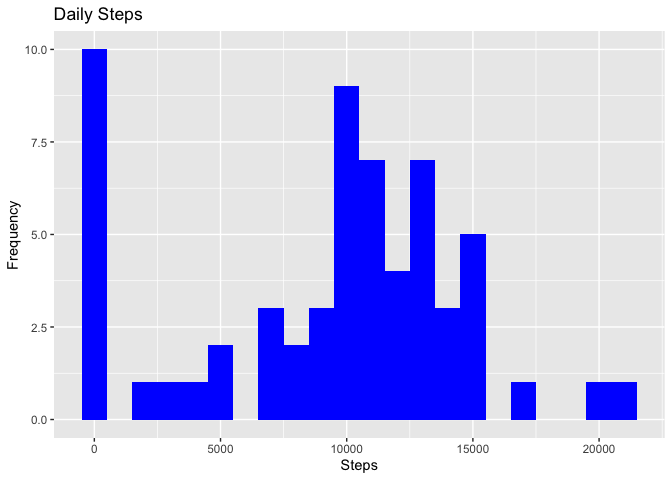
\includegraphics{PA1_template_files/figure-latex/unnamed-chunk-11-1.pdf}

\begin{longtable}[]{@{}lll@{}}
\toprule
Type of Estimate & Mean\_Steps & Median\_Steps\tabularnewline
\midrule
\endhead
First Part (with na) & 10765 & 10765\tabularnewline
Second Part (fillin in na with median) & 9354.23 & 10395\tabularnewline
\bottomrule
\end{longtable}

\hypertarget{are-there-differences-in-activity-patterns-between-weekdays-and-weekends}{%
\subsection{Are there differences in activity patterns between weekdays
and
weekends?}\label{are-there-differences-in-activity-patterns-between-weekdays-and-weekends}}

\begin{enumerate}
\def\labelenumi{\arabic{enumi}.}
\tightlist
\item
  Create a new factor variable in the dataset with two levels --
  ``weekday'' and ``weekend'' indicating whether a given date is a
  weekday or weekend day.
\end{enumerate}

\begin{Shaded}
\begin{Highlighting}[]
\CommentTok{# Just recreating activityDT from scratch then making the new factor variable. (No need to, just want to be clear on what the entire process is.) }
\NormalTok{activityDT <-}\StringTok{ }\NormalTok{data.table}\OperatorTok{::}\KeywordTok{fread}\NormalTok{(}\DataTypeTok{input =} \StringTok{"data/activity.csv"}\NormalTok{)}
\NormalTok{activityDT[, date }\OperatorTok{:}\ErrorTok{=}\StringTok{ }\KeywordTok{as.POSIXct}\NormalTok{(date, }\DataTypeTok{format =} \StringTok{"%Y-%m-%d"}\NormalTok{)]}
\NormalTok{activityDT[, }\StringTok{`}\DataTypeTok{Day of Week}\StringTok{`}\OperatorTok{:}\ErrorTok{=}\StringTok{ }\KeywordTok{weekdays}\NormalTok{(}\DataTypeTok{x =}\NormalTok{ date)]}
\NormalTok{activityDT[}\KeywordTok{grepl}\NormalTok{(}\DataTypeTok{pattern =} \StringTok{"Monday|Tuesday|Wednesday|Thursday|Friday"}\NormalTok{, }\DataTypeTok{x =} \StringTok{`}\DataTypeTok{Day of Week}\StringTok{`}\NormalTok{), }\StringTok{"weekday or weekend"}\NormalTok{] <-}\StringTok{ "weekday"}
\NormalTok{activityDT[}\KeywordTok{grepl}\NormalTok{(}\DataTypeTok{pattern =} \StringTok{"Saturday|Sunday"}\NormalTok{, }\DataTypeTok{x =} \StringTok{`}\DataTypeTok{Day of Week}\StringTok{`}\NormalTok{), }\StringTok{"weekday or weekend"}\NormalTok{] <-}\StringTok{ "weekend"}
\NormalTok{activityDT[, }\StringTok{`}\DataTypeTok{weekday or weekend}\StringTok{`} \OperatorTok{:}\ErrorTok{=}\StringTok{ }\KeywordTok{as.factor}\NormalTok{(}\StringTok{`}\DataTypeTok{weekday or weekend}\StringTok{`}\NormalTok{)]}
\KeywordTok{head}\NormalTok{(activityDT, }\DecValTok{10}\NormalTok{)}
\end{Highlighting}
\end{Shaded}

\begin{verbatim}
##     steps       date interval Day of Week weekday or weekend
##  1:    NA 2012-10-01        0      Monday            weekday
##  2:    NA 2012-10-01        5      Monday            weekday
##  3:    NA 2012-10-01       10      Monday            weekday
##  4:    NA 2012-10-01       15      Monday            weekday
##  5:    NA 2012-10-01       20      Monday            weekday
##  6:    NA 2012-10-01       25      Monday            weekday
##  7:    NA 2012-10-01       30      Monday            weekday
##  8:    NA 2012-10-01       35      Monday            weekday
##  9:    NA 2012-10-01       40      Monday            weekday
## 10:    NA 2012-10-01       45      Monday            weekday
\end{verbatim}

\begin{enumerate}
\def\labelenumi{\arabic{enumi}.}
\setcounter{enumi}{1}
\tightlist
\item
  Make a panel plot containing a time series plot (i.e.~𝚝𝚢𝚙𝚎 = ``𝚕'') of
  the 5-minute interval (x-axis) and the average number of steps taken,
  averaged across all weekday days or weekend days (y-axis). See the
  README file in the GitHub repository to see an example of what this
  plot should look like using simulated data.
\end{enumerate}

\begin{Shaded}
\begin{Highlighting}[]
\NormalTok{activityDT[}\KeywordTok{is.na}\NormalTok{(steps), }\StringTok{"steps"}\NormalTok{] <-}\StringTok{ }\NormalTok{activityDT[, }\KeywordTok{c}\NormalTok{(}\KeywordTok{lapply}\NormalTok{(.SD, median, }\DataTypeTok{na.rm =} \OtherTok{TRUE}\NormalTok{)), .SDcols =}\StringTok{ }\KeywordTok{c}\NormalTok{(}\StringTok{"steps"}\NormalTok{)]}
\NormalTok{IntervalDT <-}\StringTok{ }\NormalTok{activityDT[, }\KeywordTok{c}\NormalTok{(}\KeywordTok{lapply}\NormalTok{(.SD, mean, }\DataTypeTok{na.rm =} \OtherTok{TRUE}\NormalTok{)), .SDcols =}\StringTok{ }\KeywordTok{c}\NormalTok{(}\StringTok{"steps"}\NormalTok{), by =}\StringTok{ }\NormalTok{.(interval, }\StringTok{`}\DataTypeTok{weekday or weekend}\StringTok{`}\NormalTok{)] }

\KeywordTok{ggplot}\NormalTok{(IntervalDT , }\KeywordTok{aes}\NormalTok{(}\DataTypeTok{x =}\NormalTok{ interval , }\DataTypeTok{y =}\NormalTok{ steps, }\DataTypeTok{color=}\StringTok{`}\DataTypeTok{weekday or weekend}\StringTok{`}\NormalTok{)) }\OperatorTok{+}\StringTok{ }\KeywordTok{geom_line}\NormalTok{() }\OperatorTok{+}\StringTok{ }\KeywordTok{labs}\NormalTok{(}\DataTypeTok{title =} \StringTok{"Avg. Daily Steps by Weektype"}\NormalTok{, }\DataTypeTok{x =} \StringTok{"Interval"}\NormalTok{, }\DataTypeTok{y =} \StringTok{"No. of Steps"}\NormalTok{) }\OperatorTok{+}\StringTok{ }\KeywordTok{facet_wrap}\NormalTok{(}\OperatorTok{~}\StringTok{`}\DataTypeTok{weekday or weekend}\StringTok{`}\NormalTok{ , }\DataTypeTok{ncol =} \DecValTok{1}\NormalTok{, }\DataTypeTok{nrow=}\DecValTok{2}\NormalTok{)}
\end{Highlighting}
\end{Shaded}

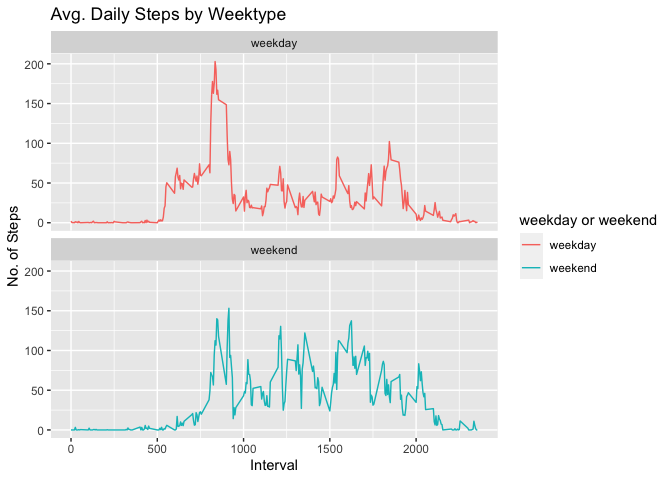
\includegraphics{PA1_template_files/figure-latex/unnamed-chunk-13-1.pdf}

\end{document}
